% LICENSE: see LICENCE
\section{Single-Frequency Networks}
\subsection{Requirements}
The DAB standard has been designed to enable the creation of transmission
networks where several transmitters share the same frequency, and send the same
signal synchronously. Such networks are called ``Single-Frequency Networks''.
Each transmitter needs to be fed the same multiplex stream, which must include
timing information required for synchronisation. This timing information implies
that a time reference must be installed at each transmitter.

The requirements for a SFN can therefore be summarised in three points:
\begin{itemize}
    \item The signal must be \emph{identical} for each transmitter. This
        requires a common multiplexers, and a distribution network that carries
        the ETI to all modulators.
    \item All transmitters must transmit on the \emph{same frequency}. The modulators
        require a frequency reference.
    \item The signal must be transmitted at the \emph{same time}, which requires
        a time reference at each site. It also implies that the ETI stream must
        contain timestamps.
\end{itemize}


The figure~\ref{fig:txchain-sfn} shows a SFN setup with two transmitters.

\begin{figure}[h]
    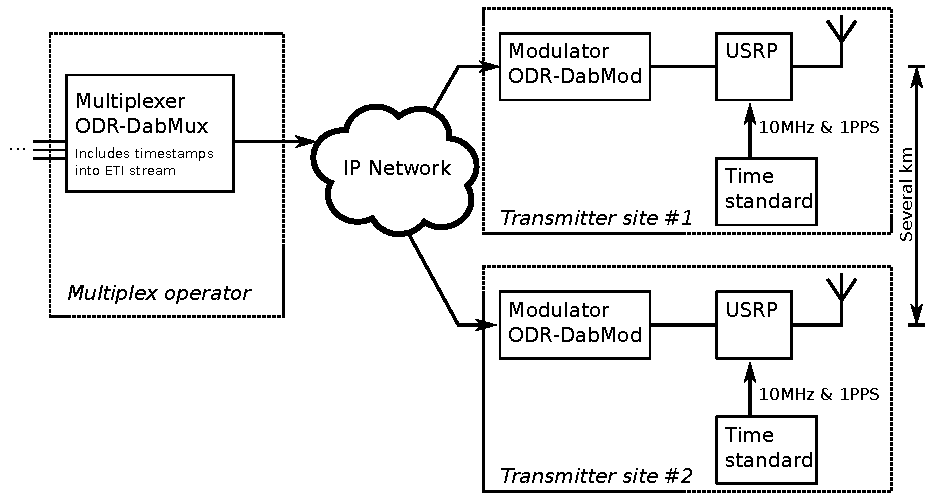
\includegraphics[width=\textwidth]{figures/txchain-sfn.pdf}
    \caption{This outline for a SFN shows two transmission sites.}
    \label{fig:txchain-sfn}
\end{figure}

\sidenote{Explain requirements on system time, NTP}

\subsection{Multiplexer Configuration}
On the ODR-DabMux configuration, there are not many options that are specific to
an SFN setup.
Most importantly, the timestamp feature must be enabled using the ``tist'' option in
the ``general'' section.

Furthermore, it is recommended to use the ZeroMQ transport between the
multiplexer and the modulators, which can be enabled in the ``outputs'' section.
Care has to be taken to have an output that slows ODR-DabMux down to nominal
rate. The ZeroMQ output alone does not enforce this. The following listing shows
the relevant options we just covered.

\begin{lstlisting}
general {
    tist true
    ...
}

...

outputs {
    ; Accept connections on all interfaces, on port 9100
    zmq  "zmq+tcp://*:9100"
    ; This throttles muxing down to nominal rate
    throttle "simul://"
}
\end{lstlisting}

\subsection{Modulator Configuration}
Since the modulator has to ensure that the three SFN requirements are satisfied,
its configuration is more complex.

We will assume, in this explanation, that one of the following USRP devices is
used: USRP2, USRP B100, USRP B200. Other devices also support the necessary time
and frequency synchronisation, but they have not been well tested. These USRP
devices can accept different sources for the reference clock:
\begin{itemize}
    \item The default ``internal'' source uses the non-disciplined
        clock generator inside the USRP. It is not suitable for SFN.
    \item The ``external'' source corresponds to the SMA connector on
        the USRP. A 10MHz signal from an external source must be connected to
        it.
    \item The optional GPSDO that can be mounted inside the USRP, and is
        selected as source with the ``gpsdo'' setting.
\end{itemize}

For the time reference, the ``pps\_source'' option is used. Possible values are
``none'', ``external'' and ``gpsdo'', with analogous meaning as for the
reference clock.

In case the USRP is connected to external references, the relevant configuration
would be as follows:

\begin{lstlisting}
[uhdoutput]
refclk_source=external
pps_source=external
\end{lstlisting}

These settings alone do not tell the modulator to enable synchronisation of the
transmission, they only select how the USRP is configured. To enable timestamp
decoding and the frame synchronisation logic in ODR-DabMod, the following
settings must also be set:

\begin{lstlisting}
[delaymanagement]
synchronous=1

; The constant offset to be added to the TIST, in seconds
offset=2.0
\end{lstlisting}

The ``offset'' setting deserves some further explanations. The ETI data stream
contains TIST information, from which a time-stamp for each ETI frame can be
derived. Each ETI frame ($24$\ms interval) is therefore associated with a
precise point in time that defines the time of transmission of the corresponding
transmission frame.\footnote{It is slightly more complex, because one
    transmission frame is composed of several ETI frames in some
    transmission modes, but the principle stays the same. It suffices for this
    explanation that we can derive the transmission time from the TIST
information.} The TIST information is set to current time at ETI frame
generation, and does not take in account the propagation delay across the
distribution network. Therefore, we need to add an offset, called $\delta$, to
the TIST to define transmission time.

\[
t_{transmission} = t_{TIST} + \delta
\]

If this offset is set to a higher value, there will be a bigger delay (measured
in absolute time) between the point in time a frame is multiplexed and the point
in time the frame is transmitted. More frames therefore will be buffered in
the ODR-DabMod input, increasing robustness against network latency
fluctuations.

The offset already has two functions: it compensates for network delay and
allows a trade-off between delay and robustness. But it also serves a third
purpose: When doing coverage planning for an SFN, it is necessary to be able to
control the relative delay between transmitters in the order of milliseconds.
This tuning of relative delay is included in the ``offset'' setting. We can
therefore rewrite the above equation as:

\[
    t_{transmission} = t_{TIST} + \delta_{network} + \delta_{planning}
\]
\[
    \delta_{offset} = \delta_{network} + \delta_{planning}
\]

When using the ZeroMQ input, the \verb+max_frames_queued+ setting must be
large enough to contain enough ETI frames to accommodate the offset.

\subsection{Using ODR LEA-M8F GPSDO board}

The ODR GPSDO board integrating a u-blox LEA-M8F module can be used as time and
frequency reference for the USRP B200. \sidenote{TODO: Add Picture}
The board design is available on the Opendigitalradio website, with
a bill of materials describing how to source the components. The PCB itself can
be manufactured in any PCB fab.

The module includes the correct pin header so that it can be mounted directly
onto the USRP B200, but also includes footprints for SMA connectors for other
usages. Communication between the PC and the GPS is possible through USB or over
UART through the B200.

The u-blox LEA-M8F module is a GPS disciplined TCXO module, with a one-pulse per
second and a reference clock output at a frequency of $30.72$ MHz. This is
different than what the normal USRP firmware expects.

Because the UART communication protocol and the reference clock frequency are
different than for the GPSDO units Ettus supports, a modified version of UHD is
necessary. This version includes new UHD sensors, used by ODR-DabMod to verify
that the GPSDO is locked properly, and different configuration settings for the
clock management PLL inside the USRP, making the USRP compatible to the
$30.72$MHz reference clock frequency.

The modified UHD version is available on the ODR GitHub\footnote{
    \url{http://www.github.com/Opendigitalradio/uhd.git}} and is used in place
of Ettus' UHD.

ODR-DabMod can be configured as follows:
\begin{lstlisting}
[uhdoutput]
refclk_source=gpsdo
pps_source=gpsdo
behaviour_refclk_lock_lost=crash
max_gps_holdover_time=600
\end{lstlisting}


\subsection{Using Ettus GPSDO}
When using the GPSDO from Ettus, which is a Jackson Labs Firefly module, no
special UHD version needs to be installed.

The configuration is:
\begin{lstlisting}
[uhdoutput]
refclk_source=gpsdo-ettus
pps_source=gpsdo
behaviour_refclk_lock_lost=crash
max_gps_holdover_time=600
\end{lstlisting}

% vim: spl=en spell tw=80 et
